                %%%%%%%%%%%%%%%%%%%%%%%%%%%%%%%%%%%%%%%%%
% Beamer Presentation
% LaTeX Template
% Version 1.0 (10/11/12)
%
% This template has been downloaded from:
% http://www.LaTeXTemplates.com
%
% License:
% CC BY-NC-SA 3.0 (http://creativecommons.org/licenses/by-nc-sa/3.0/)
%
%%%%%%%%%%%%%%%%%%%%%%%%%%%%%%%%%%%%%%%%%

%----------------------------------------------------------------------------------------
%   PACKAGES AND THEMES
%----------------------------------------------------------------------------------------

\documentclass{beamer}

\mode<presentation> {

% The Beamer class comes with a number of default slide themes
% which change the colors and layouts of slides. Below this is a list
% of all the themes, uncomment each in turn to see what they look like.

%\usetheme{default}
%\usetheme{AnnArbor}
%\usetheme{Antibes}
%\usetheme{Bergen}
%\usetheme{Berkeley}
%\usetheme{Berlin}
%\usetheme{Boadilla}
%\usetheme{CambridgeUS}
%\usetheme{Copenhagen}
%\usetheme{Darmstadt}
%\usetheme{Dresden}
%\usetheme{Frankfurt}
%\usetheme{Goettingen}
%\usetheme{Hannover}
%\usetheme{Ilmenau}
%\usetheme{JuanLesPins}
%\usetheme{Luebeck}
\usetheme{Madrid}
%\usetheme{Malmoe}
%\usetheme{Marburg}
%\usetheme{Montpellier}
%\usetheme{PaloAlto}
%\usetheme{Pittsburgh}
%\usetheme{Rochester}
%\usetheme{Singapore}
%\usetheme{Szeged}
%\usetheme{Warsaw}

% As well as themes, the Beamer class has a number of color themes
% for any slide theme. Uncomment each of these in turn to see how it
% changes the colors of your current slide theme.

%\usecolortheme{albatross}
%\usecolortheme{beaver}
%\usecolortheme{beetle}
%\usecolortheme{crane}
%\usecolortheme{dolphin}
%\usecolortheme{dove}
%\usecolortheme{fly}
%\usecolortheme{lily}
%\usecolortheme{orchid}
%\usecolortheme{rose}
%\usecolortheme{seagull}
%\usecolortheme{seahorse}
%\usecolortheme{whale}
%\usecolortheme{wolverine}

%\setbeamertemplate{footline} % To remove the footer line in all slides uncomment this line
%\setbeamertemplate{footline}[page number] % To replace the footer line in all slides with a simple slide count uncomment this line

%\setbeamertemplate{navigation symbols}{} % To remove the navigation symbols from the bottom of all slides uncomment this line
}

\usepackage{graphicx} % Allows including images
\usepackage{booktabs} % Allows the use of \toprule, \midrule and \bottomrule in tables
\usepackage{amsmath}

%----------------------------------------------------------------------------------------
%   TITLE PAGE
%----------------------------------------------------------------------------------------

\title[Short title]{Baselines and ER in policy gradient learning} % The short title appears at the bottom of every slide, the full title is only on the title page

\author{Nikita Petrenko} % Your name

\date{\today} % Date, can be changed to a custom date

\begin{document}

\begin{frame}
\titlepage % Print the title page as the first slide
\end{frame}

\begin{frame}
\frametitle{Overview} % Table of contents slide, comment this block out to remove it
\tableofcontents % Throughout your presentation, if you choose to use \section{} and \subsection{} commands, these will automatically be printed on this slide as an overview of your presentation
\end{frame}

%----------------------------------------------------------------------------------------
%   PRESENTATION SLIDES
%----------------------------------------------------------------------------------------

%------------------------------------------------
\section{Overview of common policy gradient methods} % Sections can be created in order to organize your presentation into discrete blocks, all sections and subsections are automatically printed in the table of contents as an overview of the talk


\begin{frame}[t]
\frametitle{Common methods of PG learning}

Unnormalized discounted state distribution: $\rho_\pi :=  \sum_{t=0}^\infty \gamma^t P(s_0 \rightarrow s | t)$ 

\begin{itemize}

\item A3C: $\nabla_\theta V(s) = E_{\rho_\pi, \pi}(\nabla \log \pi_\theta (a) * (r(s,a) + V(s') - V(s)))$ 
\\basic algorithm which exhibits high gradient variance and inability to learn on off-policy data (including Experience Replay)

\item A3C with Importance Sampling (IS): \[ \nabla_\theta V(s) = E_{traj \sim \pi_{\theta'}} \left[ \dfrac{P(traj)}{P'(traj)} \nabla \log \pi_\theta (a) (r(s,a) + V(s') - V(s)) \right] \]
\\Unbiased estimation of policy gradient with off-policy data. However, it suffers from possibly infinite variance of density ratios if behavioral policy (the one that collected samples) and agent policy are too different.
\\In MDP setting, 

\begin{equation}
\dfrac{P(traj)}{P'(traj)} = \dfrac{p(s_0) \pi (a_0 | s_0) p(s_1 | a_0, s_0)
...} {p(s_0) \pi' (a_0 | s_0) p(s_1 | a_0, s_0)
...} = \prod_{t=0}^{T-1} \dfrac{\pi (a_t | s_t)} {\pi' (a_t | s_t)}
\end{equation}

\end{itemize}
\end{frame}

\begin{frame}[t]
\frametitle{Common methods of PG learning}
\begin{itemize}

\item TRPO: derives lower bound on policy improvement thus allowing to make several gradient update steps on sampled trajectories. Improves sample efficiency significantly.

\end{itemize}
\end{frame}

%------------------------------------------------
\section{Q-prop}
%------------------------------------------------
\subsection{Features}

\begin{frame}[t]
\frametitle{Q-prop}

Main features:
\begin{itemize}
\item Unbiased, low variance gradient
\item On-policy actor with control variate
\item Off-policy critic
\item Ability to use TRPO for policy updates
\end{itemize}

\vspace{4mm}
Limitations:
\begin{itemize}
\item Continuous control only
\end{itemize}

\end{frame}

\subsection{Q-prop estimator}
\begin{frame}[t]
\frametitle{Q-prop estimator}
Variance reduction through action-dependent control variates\\
 
$\overline{f} (x,a) = f(x,\overline{a}) + \nabla_a f(x, a) (a - \overline{a})$

$\mu_\theta(s) = E_{\pi_\theta(a|s)} (a)$

\begin{theorem}[Q-prop gradient]
$\forall f, \overline{a}, \eta$
\begin{multline}
\nabla_{\theta} J = E_{\rho_\pi, \pi} \left[ \nabla_{\theta} log \pi_\theta ( a_t | s_t) (Q(s_t, a_t) - \eta(s_t) \overline{f} (s_t,a_t)) \right] + \\ + E_{\rho_\pi} \left[ \eta(s_t) \nabla_a f(s_t, a) |_{a=\overline{a_t}} 
\nabla_\theta \mu_\theta(s_t)
\right]
\end{multline} 
\end{theorem}

Suggested choice: 
\begin{itemize}
\item $f = Q_w$ -- off-policy critic, same as in DDPG
\item $\overline{a} = \mu_\theta(s_t)$
\end{itemize}

Compare it to DDPG policy gradient:
\\$E_{data} \left[ \nabla_a Q_w (s_t, a) |_{a=\mu_\theta(s_t)} 
\nabla_\theta \mu_\theta(s_t) \right]$

\end{frame}

% ----------------------
\begin{frame}[t]
\frametitle{Proof}

\begin{equation}
g(\theta) = E_{\rho_\pi, \pi} \left[ \nabla_\theta log \pi(a_t | s_t) \overline{f} (s_t, a_t) \right] =
\end{equation}

\begin{equation}
= E_{\rho_\pi, \pi} \left[ \nabla_\theta log \pi(a_t | s_t) (f (s_t, \overline{a_t}) + 
\nabla_a f(s_t, a) |_{a=\overline{a_t}} (a_t - \overline{a_t})) \right]
\end{equation}

\begin{equation}
= E_{\rho_\pi, \pi} \left[ \nabla_\theta log \pi(a_t | s_t) ( 
\nabla_a f(s_t, a) |_{a=\overline{a_t}} a_t) \right]
\end{equation}

\begin{equation}
= E_{\rho_\pi} \left[ \int_{A} \nabla_\theta \pi(a_t | s_t) ( 
\nabla_a f(s_t, a) |_{a=\overline{a_t}} a_t) da_t \right]
\end{equation}

\begin{equation}
= E_{\rho_\pi} \left[ \nabla_a f(s_t, a) |_{a=\overline{a_t}} \int_{A} \nabla_\theta \pi(a_t | s_t) a_t da_t \right]
\end{equation}

\begin{equation}
= E_{\rho_\pi} \left[ \nabla_a f(s_t, a) |_{a=\overline{a_t}} \nabla_\theta E_{\pi(a_t | s_t)} a_t \right] = E_{\rho_\pi} \left[ \nabla_a f(s_t, a) |_{a=\overline{a_t}} \nabla_\theta \mu_\theta(a_t) \right]
\end{equation}

\end{frame}

\subsection{Variance analysis}
\begin{frame}[t]
\frametitle{Variance analysis}
Our final gradient estimator:
\begin{multline*}
\nabla_{\theta} J = E_{\rho_\pi, \pi} \left[ \nabla_{\theta} log \pi_\theta ( a_t | s_t) (A(s_t, a_t) - \eta(s_t) \overline{A_w} (s_t,a_t)) \right] + \\ + E_{\rho_\pi} \left[ \eta(s_t) \nabla_a Q_w(s_t, a) |_{a=\mu_\theta(s_t)} 
\nabla_\theta \mu_\theta(s_t)
\right]
\end{multline*}
Authors analyze 

\begin{equation*}
\begin{aligned}
Var^* &= E_{\rho_\pi} \left[ Var_{a_t}(A(s_t,a_t) - \eta(s_t) \overline{A_w} (s_t,a_t) )\right]&&\\
      &= Var + E_{\rho_\pi} \left[ \eta(s_t) Cov_{a_t} (A(s_t, a_t), \overline{A}(s_t, a_t)) + \eta^2(s_t) Var(\overline{A}(s_t, a_t)) \right]&&\\
\end{aligned}
\end{equation*}

\begin{equation*}
\begin{aligned}
 Cov_{a_t} (A(s_t, a_t), \overline{A}(s_t, a_t)) &= E_\pi (A(s_t,a_t) \overline{A}(s_t, a_t))&&\\
 Var_{a_t} (\overline{A}(s_t, a_t)) &= E_\pi (\overline{A}^2(s_t, a_t))&&\\
 &= \nabla_a Q_w(s_t, a) |_{a=\mu_\theta(s_t)}^T \Sigma_\theta(s_t) \nabla_a Q_w(s_t, a) |_{a=\mu_\theta(s_t)}&&\\
\end{aligned}
\end{equation*}

where $\Sigma_\theta(s_t)$ is a covariance matrix of stochastic policy $\pi_\theta$ at state $s_t$
\\ Therefore, optimal $\eta^*(s_t) = Cov(A,\overline{A})/Var(\overline{A})$ can be approximated with single sample


\end{frame}

\begin{frame}[t]
\frametitle{Choice of $\eta$}
\begin{itemize}
\item $\eta(s_t) = Cov(A,\overline{A})/Var(\overline{A})$ leads to Adaptive Q-prop. However, its variance can be big itself if we're using single sample estimation of Cov.
\item Conservative Q-prop: \\
$\eta(s_t) =
	\begin{cases}
		1 & \text{$Cov > 0$}\\
		0 & \text{...}
	\end{cases}$
\item Aggressive Q-prop: \\
$\eta(s_t) = sgn(Cov)$
	

\end{itemize}

\end{frame}

\subsection{Value function estimation}
\begin{frame}[t]
\frametitle{Value function estimation}
Q-function estimation for control variate:\\
\vspace{1mm}

$T_\pi[Q](s,a) := r(s,a) + E_\pi[Q(s',a') | s,a]$\\

$w \leftarrow argmin_w \| T_\pi[Q_{w'}] - Q_w \|_2$\\
$ w' \leftarrow \tau w' + (1-\tau) w, \tau = 0.999$

\vspace{4mm}

Value function estimation:\\
\vspace{1mm}
$\phi \leftarrow argmin \sum \| V_\phi(s_n) - (r + V_\phi(s_n')) \|_2$;\\
subj. to $\frac{1}{N} \sum_{n=1}^N \frac{\| V_\phi(s_n) - V_{\phi_{old}}(s_n) \|_2} {2\sigma^2}$\\
$(s_n,s_n') \sim MDP_\pi$


\end{frame}

\begin{frame}[t]

Continuous control of bias-variance tradeoff (GAE($\lambda$)):\\
\vspace{1mm}
$Q^\lambda (s_t,a_t) = (1-\lambda) \sum_{k=0}^{\infty} \lambda^k \left[ \sum_{m=0}^{k-1} \gamma^m r(s_{t+m}, a_{t+m}) + \gamma^{k} V_\phi  (s_{t+k}, a_{t+k}) \right]$

\vspace{1.5mm}
$\lambda \rightarrow 1 \Rightarrow Q^\lambda \rightarrow R$\\
$\lambda \rightarrow 0 \Rightarrow Q^\lambda \rightarrow V_\phi$\\

\vspace{4mm}
Advantage for CV:\\
$\overline{A_w} (s_t,a_t) = (a - \mu(\theta) )\nabla_a Q(s_t,a)|_{a=\mu(\theta)}$
\end{frame}

\begin{frame}[t]
\frametitle{Algorithm}
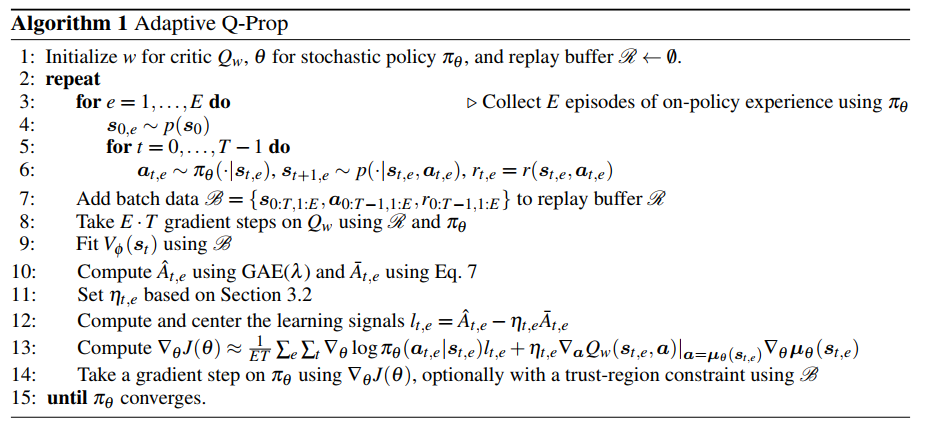
\includegraphics[scale=0.35]{q-prop-algo}
\end{frame}

\subsection{Empirical Results}
\begin{frame}[t]
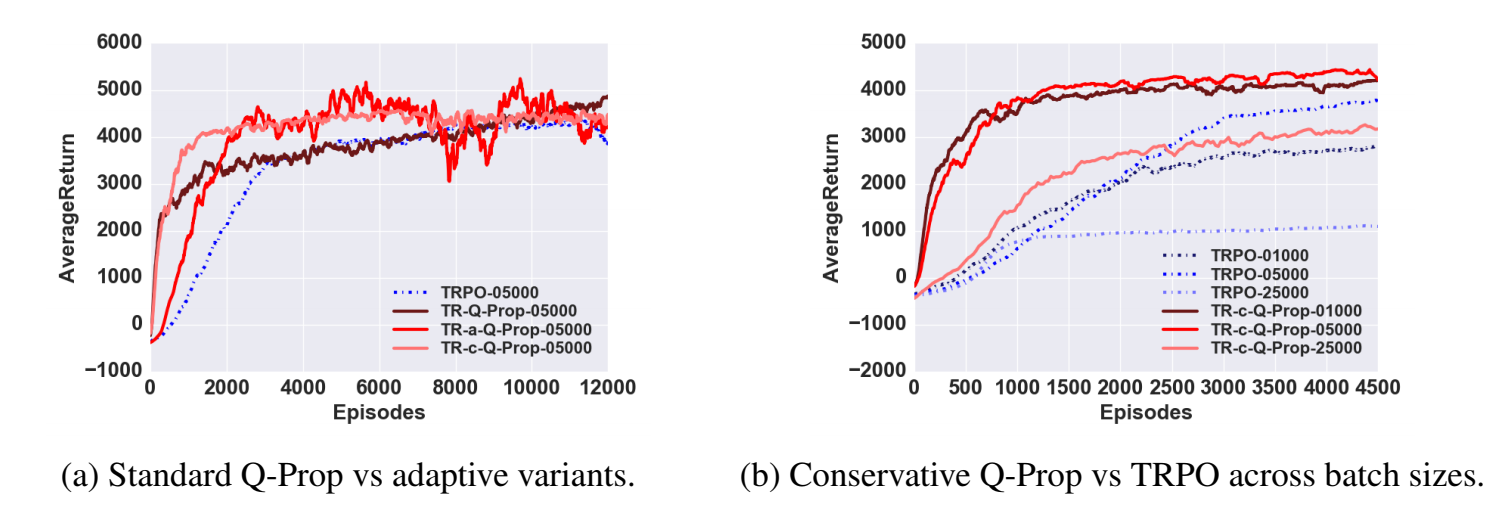
\includegraphics[scale=0.23]{q-prop1}
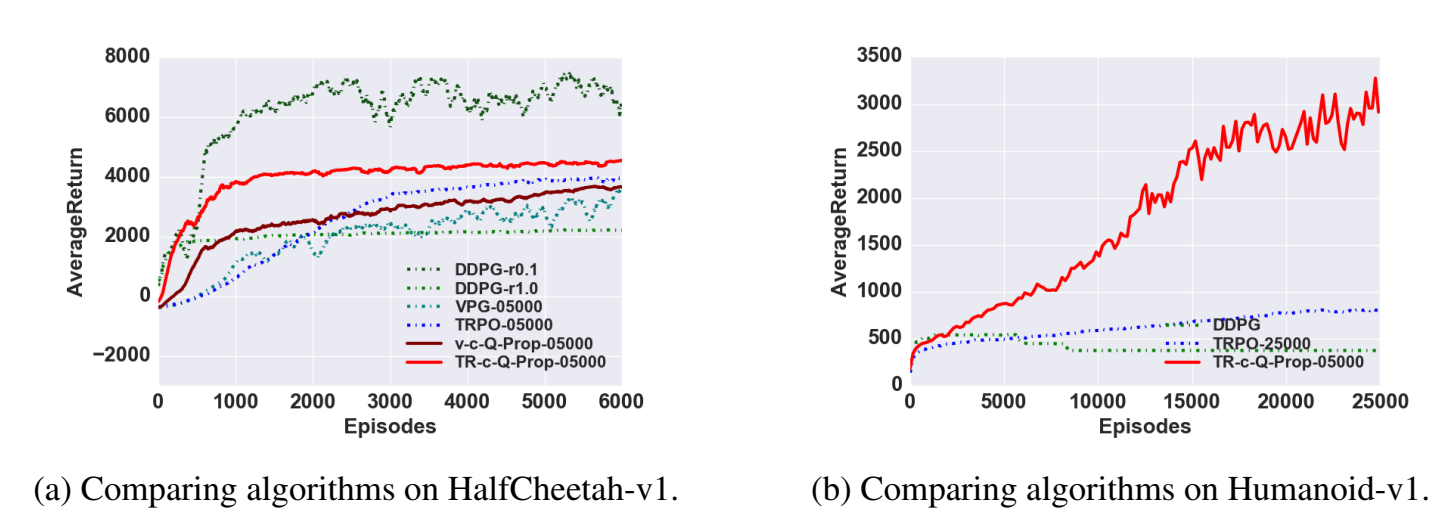
\includegraphics[scale=0.23]{q-prop2}
\end{frame}

\begin{frame}
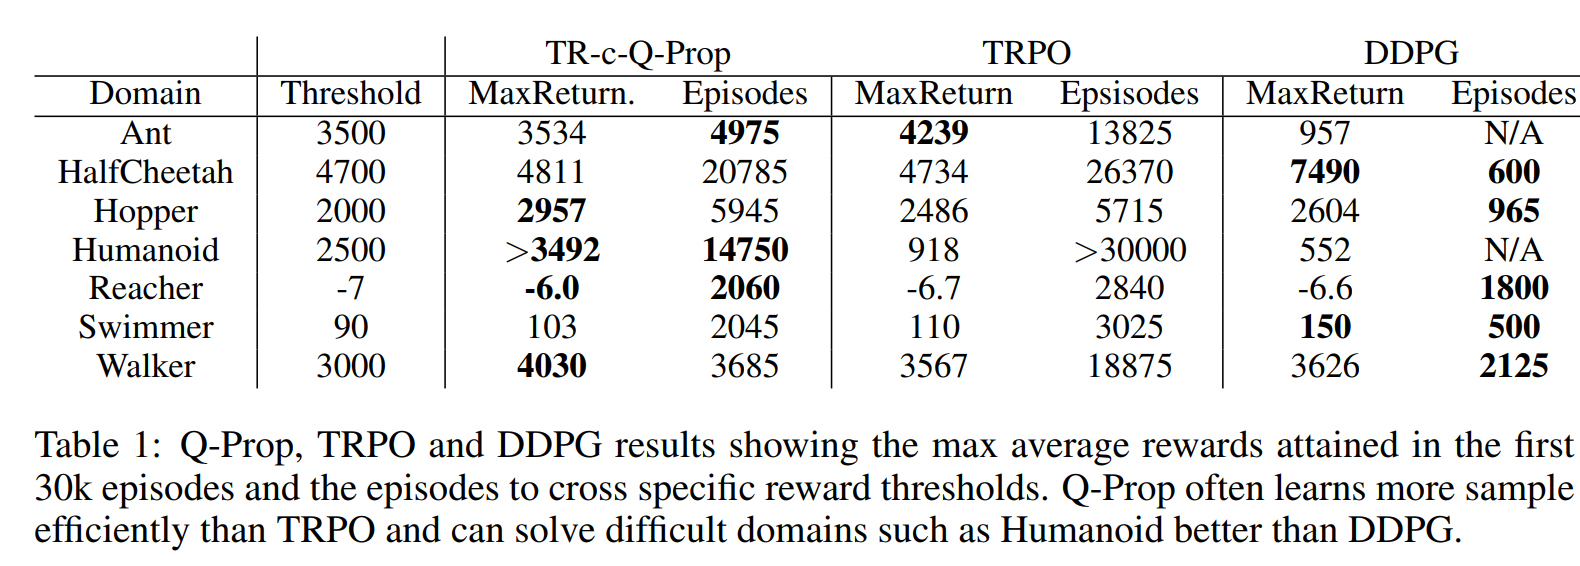
\includegraphics[scale=0.21]{q-prop3}
\end{frame}

\section{Unifying Policy Gradient And Actor-Critic}

\begin{frame}[t]
\frametitle{Unifying Policy Gradient And Actor-Critic}

Proposed extention:
\begin{multline*}
\nabla_{\theta} J \simeq \alpha E_{\rho_\pi, \pi} \left[ \nabla_{\theta} log \pi_\theta ( a_t | s_t) (A(s_t, a_t) - \eta \overline{A_w} (s_t,a_t)) \right] + \\ + \eta E_{\rho_{CR}} \left[ \nabla_a Q_w(s_t, a) |_{a=\mu_\theta(s_t)} 
\nabla_\theta \mu_\theta(s_t)
\right]
\end{multline*}
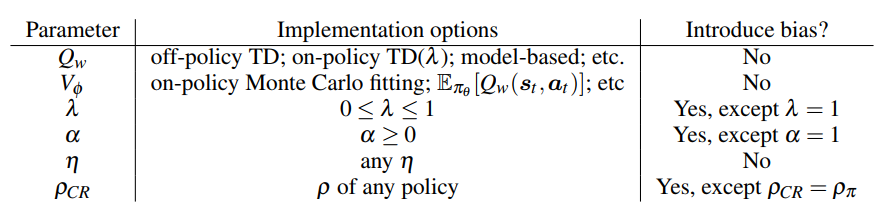
\includegraphics[scale=0.37]{extention}

\end{frame}

\end{document}